\chapter{Detector Design and Construction Organization}
\label{vl:tc-overview}

The design and construction of the \dword{dune} detector elements is 
carried out by the international \dword{dune} Project.  \dword{dune}
collaboration management is responsible for overseeing this portion 
of the \dword{lbnf-dune} and ensuring its successful execution.  
The high-level \dword{dune} management team consisting of the 
co-spokespersons, \dword{tcoord}, and \dword{rcoord} is responsible 
for the day-to-day administration of the project.  

\section{DUNE Work Flow}
\label{sec:workflow}

Figure~\ref{fig:DUNE_workflow} indicates the time-sequenced set of 
activities needed to implement the \dword{dune} far \dwords{detmodule}.
The \dword{dune} project has direct responsibility for the design, 
prototyping, fabrication, and transportation of the \dword{fd} 
elements.  These activities are managed by the \dword{dune} \dword{tc} 
organization under the direction of the \dword{tcoord}.  Activities at 
or in the vicinity of \dword{surf} are managed by the on-site integration and
installation team under the direction of the \dword{ipd} as described 
in Chapter~\ref{ch:tc-jpo}.  These activities include the receipt,
processing, installation, and operation of the detector components.            
\begin{dunefigure}[\dword{dune} work flow]{fig:DUNE_workflow}
  {\dword{dune} work flow.}
  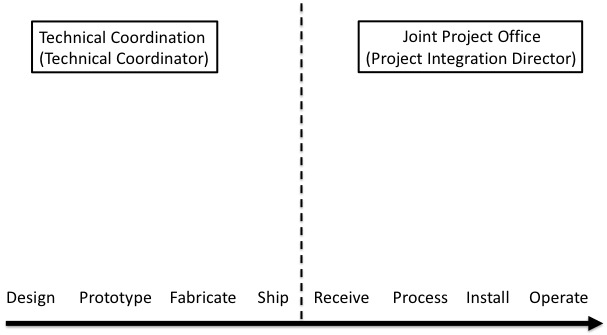
\includegraphics[width=0.99\textwidth]{DUNE_workflow}
\end{dunefigure}

Although responsibilities for the two sets of time-ordered activities 
are clearly delineated, both management teams have roles in supporting
the activities that do not fall under their direct responsibility.  The 
integration and installation team interacts directly with the \dword{dune} 
project team through detector design, prototyping, and construction to 
ensure that fabricated detector elements are properly integrated within 
the supporting infrastructure.  Conversely, the \dword{dune} project team %sm chg anne
supports the integration and installation activies at \dword{surf} by providing 
some of the dedicated resources (both personnel and equipment) necessary 
for carrying out these activities.  Ensuring proper installation and 
commissioning of the detector elements remains a \dword{dune} project
responsibility even while the global coordination of integration and 
installation activities is managed through the on-site organization.  

The \dword{dune} project has already completed an initial round of design 
and prototyping activities culminating in the construction and operation 
of the \dword{protodune} detectors.  Moving forward, the project is 
updating detector component designs to account for lessons learned from 
the \dword{protodune} experience.  Upon finalization of the designs, the 
project will construct first production versions of all components, which 
will be installed and operated in a second phase of \dword{protodune} 
operations prior to the start of full-scale production.  The operation 
of the \dword{protodune2} detectors will follow roughly two years after
the end of operations for the corresponding \dword{protodune} detectors.
In a few cases, the production of long lead-time components will need to 
be started in parallel with the operation of first production components 
in \dword{protodune2}.

\section{DUNE Consortia}
\label{sec:consortia}

Construction of the \dword{dune} far \dwords{detmodule} is carried out by 
``consortia of collaboration institutions'' who assume responsibility for 
detector subsystems.  Each consortium plans and executes the construction, 
installation and commissioning of its subsystem.

Management of each consortium is through an overall consortium leader and  
a technical lead.  The consortium leader chairs an institutional board 
composed of one representative from each of the collaborating institutions 
contributing to the activities of the consortium.  Major consortium decisions 
such as technology selections and assignment of responsibilities within 
the institutions are expected to be passed through its institutional board.  
These decisions are then passed as recommendations to the \dword{dune} 
\dword{exb}, as described in greater detail below, for formal collaboration 
approval.

Figure~\ref{fig:DUNE_consortia_org} shows a sample consortium organizational 
chart with the different parts of the internal consortium structure mandated 
by \dword{dune} collaboration management.  In addition to the pieces described 
above, the consortium in most cases needs to manage subsystem deliverables 
that are supported by more than a single funding agency.  In the sample case 
illustrated here, responsibilities for subsystem deliverables are shared 
between the USA, UK, and Switzerland (CH), where each of the 
funding agencies is expected to manage its own internal projects, which have
direct responsibility for their assigned deliverables.  To ensure coordination
between the separate internal projects contributing to the consortium, the 
technical lead is responsible for chairing a consortium project management 
board incorporating the separate managers from each of the internal projects.   
\begin{dunefigure}[\dword{dune} Internal Consortia Structure]{fig:DUNE_consortia_org}
  {\dword{dune} Internal Consortia Structure}
  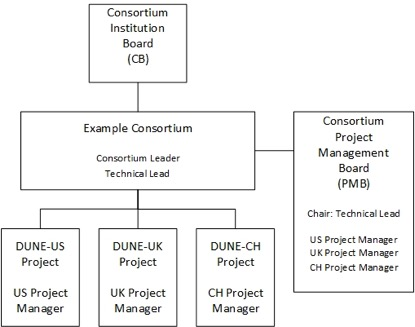
\includegraphics[width=0.99\textwidth]{DUNE_consortia_org}
\end{dunefigure}
\fixme{figure is fuzzy}

In addition to the mandated organizational pieces described here, the consortia 
incorporate additional internal structures as needed to deliver their assigned 
subsystems.  For example, working groups with convenors are typically appointed 
to focus on specific consortium activities, and steering committees are in many 
cases formed to help guide technical and strategic decisions within the consortia.
Each consortium is also expected to appoint both safety and \dword{qa} 
representatives as well as a representative with responsibility for integration 
and installation issues.  These individuals are charged with interacting directly 
with appropriate project management team personnel to ensure proper coordination 
on these topics across the consortia.        

\section{DUNE Collaboration Management}
\label{sec:dune_mgmt}

The high-level \dword{dune} collaboration management structure is shown 
in Figure~\ref{fig:DUNE_org}.  The \dword{dune} \dword{exb} is the primary
collaboration decision-making body and as such includes representatives 
from all major areas of activity within the collaboration.
\begin{dunefigure}[\dword{dune} org chart]{fig:DUNE_org}
  {\dword{dune} Organizational Chart}
  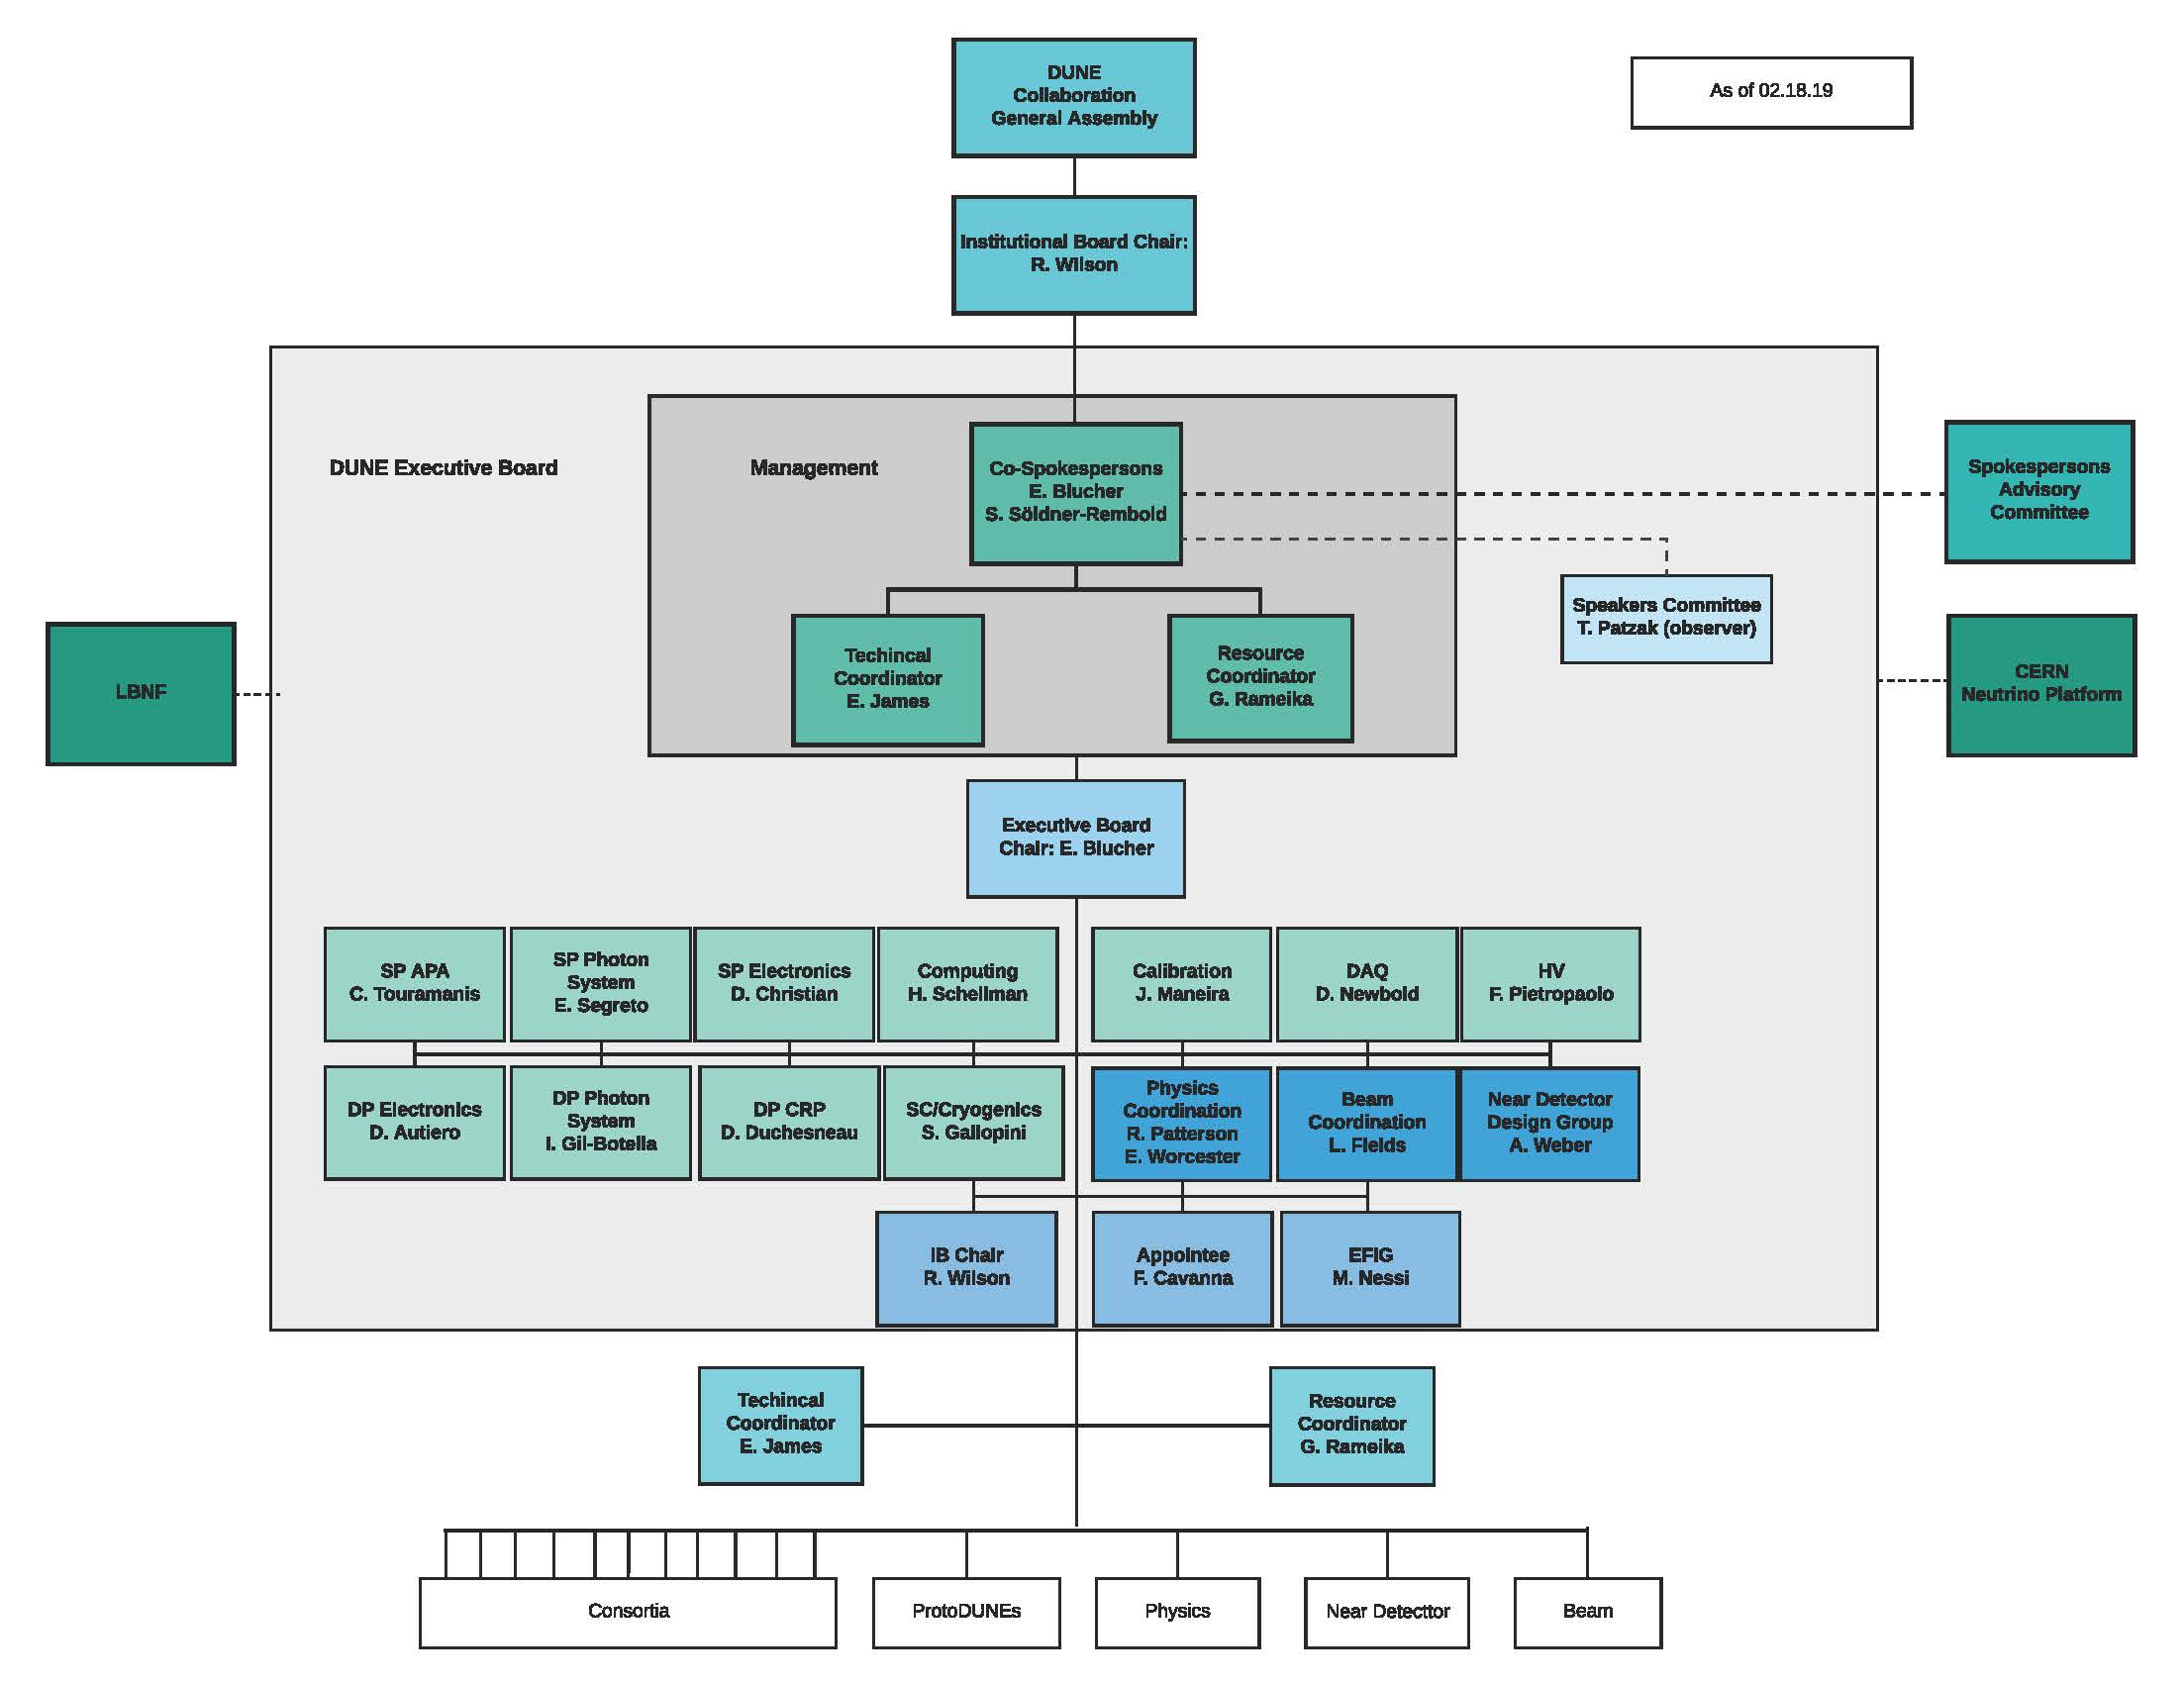
\includegraphics[width=0.99\textwidth]{DUNE_COllab_Mgmt}
\end{dunefigure}
\fixme{text in boxes should be made bigger}

Each consortium is represented on the \dword{dune} \dword{exb} by its 
consortium leader.  All collaboration decisions, especially those with potential 
impacts on the \dword{dune} scientific program or connected with the assignment 
of institutional responsibilities, pass through the \dword{exb}.  \dword{exb} 
decisions are expected to be achieved through consensus.  In cases where consensus 
cannot be obtained, decision-making responsibility passes to the co-spokespersons.

\section{Technical Coordination}
\label{sec:tc}

Because the consortia operate as self-managed entities, a strong
\dword{tc} organization is required to ensure overall integration 
of the detector elements and successful execution of the detector
construction project.  \dword{tc} areas of responsibility include 
general project oversight, systems engineering, \dword{qa} 
and safety.  In association with the support role provided by 
the consortia, \dword{tc} also works closely with the on-site 
team responsible for planning and executing the required 
detector integration and installation activities in the nearby 
surface facilities and underground detector caverns at \dword{surf} 
(see Chapter~\ref{ch:tc-jpo}).  

\dword{tc} is headed by the \dword{tcoord}, who is a \dword{fnal}
employee and is appointed jointly by the \dword{fnal} director and 
the \dword{dune} co-spokespersons.  A deputy \dword{tcoord} 
is selected from within the collaboration to assist the \dword{tc} 
in carrying out their responsibilities.

The \dword{tcoord} manages the overall detector construction project
through regular board meetings with the consortium leadership teams and 
members of the \dword{tc} organization (see Section~\ref{sec:tc}).  
These board meetings are used to identify and resolve technical issues
and serve as the primary forums for required interactions between the 
consortium leadership teams.

Technical board meetings are used to evaluate consortia design
decisions with potential impacts on overall detector performance,
ensure that interfaces between the different subsystems are well
understood and documented, and monitor the overall construction
project to identify and address both technical and interface issues 
as they arise.

Project board meetings are used to ensure that the scopes of each
consortium are fully documented with assigned institutional
responsibilities, develop and manage risks held within a global
project registry, review and manage project change requests, and
monitor the status of the overall detector construction schedule.

Any decisions generated through these board meetings are passed to 
the \dword{dune} \dword{exb} as recommendations for formal approval.
Depending on the agenda items to be discussed at a specific board 
meeting, the \dword{tcoord} will invite additional members of the 
collaboration with specific knowledge or particular expertise to 
participate.  In addition, for major decisions, the \dword{tcoord} 
will officially appoint three internal collaboration referees with 
no direct conflicts of interest to directly engage in the process.

\section{Technical Coordination Organization}
\label{sec:tco}

The \dword{tcoord} heads an organization that supports the work of 
the consortia and has responsibility for a number of major project 
support functions including:
\begin{itemize}
\item ensuring that each consortium has a well defined and complete
  scope, that interactions between consortia are sufficiently 
  well defined, and that any required scope sitting outside of the 
  consortia is provided through other sources such as collaboration
  common funds.
\item defining and documenting scope boundaries and technical 
  interfaces both between consortia and with \dword{lbnf}.  
\item developing an overall schedule with appropriate dependencies
  between activities covering all phases of the project. 
\item ensuring that appropriate engineering and safety standards 
  are developed, understood, and agreed to by all key stakeholders 
  and that these standards are conveyed to and understood by each
   consortium.
\item ensuring that all \dword{dune} requirements on \dword{lbnf} 
  for \dword{cf}, cryostat and cryogenics are clearly
  defined and agreed to by each consortium.
\item ensuring that each consortium has well developed and reviewed
  component designs, construction plans, \dword{qc} processes, and 
  safety programs.
\item monitoring the overall project schedule and the progress 
  of each consortium towards delivering its assigned scope. 
\end{itemize}
\begin{dunefigure}[\dword{dune} \dword{tc} org chart]{fig:DUNE_tc}
  {\dword{dune} \dword{tc} Organizational Chart}
  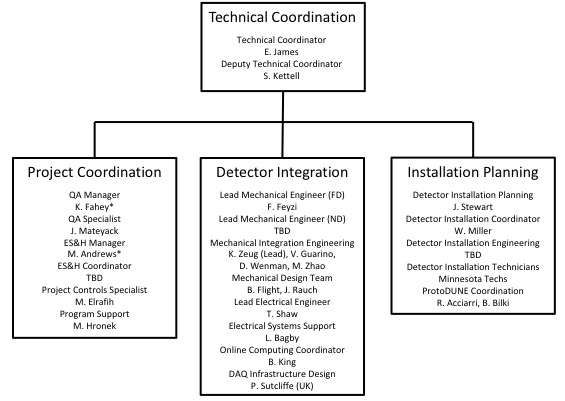
\includegraphics[width=0.99\textwidth]{DUNE_tc}
\end{dunefigure}
\fixme{figure a bit fuzzy}

The \dword{dune} \dword{tc} organizational structure is shown in 
Figure~\ref{fig:DUNE_tc}.  The structure incorporates teams with 
responsibilities in the areas of project coordination, detector integration,
and installation support.  Many of the \dword{tc} team also sit within 
the \dword{jpo} team (shown in Figure~\ref{fig:DUNE_jpo}) that ensures 
coherency in these activities across the \dword{lbnf-dune}. 

The project coordination team is led by a lead project controls
specialist, a \dword{qa} manager and an \dword{esh} manager.  The
detector integration team is directed by a lead mechanical and lead
electrical engineer, and incorporates an online-computing coordinator.
The installation support team is headed by the planning coordinators 
for activities associated with the integration and installation of 
detector components in the underground areas.  Each of the three 
teams incorporates additional personnel to support these individuals 
in carrying out their areas of responsibility.  Members of the 
\dword{tc} organization meet weekly to review project progress and 
discuss %detailed 
technical issues. 
     
Within the context of the \dword{dune} project, \dword{tc} functions 
associated with its coordination role include

\subsection{Safety}

The \dword{tcoord} is responsible for implementing the safety program
covering the \dword{dune} construction project.  The \dword{tcoord}
is supported directly in this role by the \dword{lbnf-dune} \dword{esh}
manager.  A dedicated \dword{dune} \dword{esh} coordinator sits within
the \dword{tc} organization and coordinates the \dword{dune} safety
program under the direction of the \dword{lbnf-dune} \dword{esh} manager.

The \dword{dune} construction project is carried out at many different
institutions in many different countries.  Participating institutions
sign a Memorandum of Understanding (MOU) in which they agree to abide
by the requirements of the \dword{dune} safety program.  Each of the
participating institutions assumes primary responsibility for the safe
execution of their assigned construction activities.  The \dword{dune}
\dword{esh} coordinator interacts directly with each of the participating
institutions to ensure that their saftey program meets the \dword{dune}
safety requirements.  Prior to beginning any construction activities,
the \dword{dune} \dword{esh} coordinator particpates directly in production
readiness reviews that incorporate on-site visits to confirm that the
safety program in place for those activities meets required standard.
Follow-up on-site visits by the \dword{dune} \dword{esh} coordinator over
the course of the construction period ensure are used to ensure that
program requirements are properly implemented.


\subsection{Engineering Integration}

\dword{dune} \dword{tc} works directly with the collaboration to
collect and validate the requirements associated with each detector
module.  Each detector module has a high-level set of requirements
with potential impacts on the \dword{dune} physics program under
the ownership of the \dword{dune} \dword{exb}.  Any proposed
changes to these requirements must be approved by the \dword{exb}.
Lower-level technical requirements associated with each detector
subsystem are developed by the consortia under the guidance of
the \dword{tc} detector integration team.  Appendix~\ref{sec:fdsp-coord-requirements}
contains tables summarizing the high-level requirements associated
with each of the detector modules.

Starting from these requirements, the \dword{tc} engineering
team responsible for detector integration works directly with the
\dword{dune} consortia to build and validate integrated detector
models from the designs of the individual subsystems.  The team
ensures that the detector subsystems fit together properly and
that the fully-assembled detectors meet structural requirements
associated with all operational conditions (both warm and cold).
The team is also responsible for validating that the integrated
detector designs satisfy the defined requirements needed to meet
the goals of the \dword{dune} physics program.

Integration of the full detector models within the global model
encompassing the detector caverns and supporting infrastructure
is carried out through direct interactions with the \dword{jpo}
engineering integration team.  The \dword{tc} engineering team
is responsible for validating the interfaces between \dword{dune}
detector components and supporting infrastructure pieces within
the combined model.  The \dword{tcoord} is required to sign off
on all proposed changes to the global model based on guidance
received from the lead engineers embedded within the \dword{tc}
detector integration team.

As part of these efforts, the engineering team works directly
with the consortia leadership teams to develop controlled
documents that describe the interfaces between different detector
subsystems.  These documents are placed under signature control
within the \dword{lbnf-dune} 
\dword{edms}.  Proposed changes to interface documents must be approved
by the consortia leadership teams on both sides of the subsystem
interface as well as the \dword{tc} detector integration team.

The \dword{tc} engineering team works directly with the
\dword{lbnf-dune} systems engineer, who heads the \dword{jpo} engineering
integration team, to develop the required documents detailing the
interfaces between the \dword{lbnf} and \dword{dune} projects and the interfaces
of these projects with the \dword{lbnf-dune} installation and integration
activites at \dword{surf}.  These \dword{lbnf-dune} interface documents are
also placed under signature control within the \dword{lbnf-dune}
document management system and proposed changes require sign-offs
from both the lead \dword{lbnf-dune} systems engineer and the responsible
individuals associated with each branch of the global project
(\dword{lbnf} Project Manager, \dword{dune} \dword {tcoord}, and
\dword{ipd}).

Appendix~\ref{sec:fdsp-coord-interface} summarizes the interface documents
and provides web links for accessing the approved versions of each
in place at the time of the release of this document.

 
\subsection{Change Control and Document Management}

The \dword{dune} project follows the \dword{lbnf-dune} change control process
described in Section~\ref{sec:fdsp-change}.  The decision path for
changes that do not impact the \dword{lbnf} project or \dword{lbnf-dune}
integration and installation activities at \dword{surf} is
self-contained within the \dword{dune} collaboration management
structure.  A hierarchy of decision-making levels is defined based
on pre-determined thresholds related to the extent of the proposed
change with the most significant changes requiring \dword{dune}
\dword{exb} approval.

For document management, the \dword{dune} project relies on the \dword{lbnf-dune}
document management system administrated by the \dword{jpo}
team configuration manager.  \dword{tc} works directly with the \dword{lbnf-dune}
\dword{qa} manager to ensure that the information needed to track the history
of each detector component through construction, assembly and testing
is properly captured within the PBS database.  A dedicated \dword{dune}
\dword{qa} specialist sits within the \dword{tc} organization and coordinates the
\dword{dune} \dword{qa} program under the direction of the
\dword{lbnf-dune} \dword{qa} manager.  The \dword{dune} \dword{qa} program
is described in much greater detail in Chapter~\ref{vl:tc-QA}.

 
\subsection{Schedule and Milestones}

The lead project controls specialist within the \dword{tc} team works
directly with the \dword{dune} consortia to build schedules covering
the design, testing, and construction activities associated with their
subsystems and incorporate these within the \dword{lbnf-dune} schedule.
The project controls specialist communicates with consortia Technical
Leads on a monthy basis to track the status of activities and update
the \dword{lbnf-dune} schedule accordingly.  Milestones positioned at regular
intervals within the subsystem construction schedules are incorporated
to enable high-level tracking of these efforts.  Appendix Section~\ref{sec:fdsp-coord-controls}
contains a table summarizing key detector milestones around which the
the individual consortia schedules are constructed.

\subsection{Risk Management}

\dword{dune} \dword{tc} maintains a global registry containing both
subsystem-specific risks identified by the consortia and self-held
risks associated with overall \dword{dune} project management.  The
\dword{tcoord} uses Project Board Meetings to regularly review the
risk registery with the consortia leadership teams and define
mitigation actions as necessary to prevent identified risks from being
realized.  The \dword{tcoord} does not have direct control over
contingency funds held by the internal projects of the participating
funding agencies.  In cases of identified need, the \dword{tcoord}
works directly with the consortia leadership teams to implement risk
reduction strategies.  Identified issues that cross consortia
boundaries are discussed at Project Board Meetings and brought to the
\dword{dune} \dword{exb} if they need to be addressed at a higher
level.

Appendix~\ref{ch:tc-risks} contains a table summarizing the highest-level
risks identified by the consortia as well as the project management
risks self-held by the \dword{tc} organization.


\subsection{Review Process}

The \dword{tcoord} has primary responsibility for conducting design
and production readiness reviews covering each detector subsystem.
As described in Chapter~\ref{vl:tc-review}, reviews are coordinated
through the \dword{jpo} to ensure coherency across the entire review
process.  The deputy \dword{tcoord} sits within the \dword{jpo} team
responsible for organizing the reviews.  The full review process is
described in greater detail within Chapter~\ref{vl:tc-review}.
